\documentclass{beamer}

%Includes
\usepackage[utf8]{inputenc}
\usepackage[T1]{fontenc}
\usepackage{graphics}
\usepackage[francais]{babel}

%Thème
\usetheme{Warsaw}

%Template
\setbeamertemplate{footline}[page number]

%Informations de la page de garde
\title{\textbf{Projet Njord}\\ Topographie d'une zone \\ par communication d'une équipe de drones}
\author{Aigreault Clément, Henrio Jordan, Pham Chitin}
\date{16 Mars 2015}

%Macros
%%Permet de retirer le header (ainsi que l'espace qu'il utiliserait)
\newcommand{\rmheader}{\makeatletter\setbeamertemplate{headline}[default]\def\beamer@entrycode{\vspace*{-\headheight}}\makeatother}

\begin{document}
  %Page de garde
  {
    \makeatletter
    \setbeamertemplate{headline}[default]
    \def\beamer@entrycode{\vspace*{-\headheight}}
    \makeatother
    \begin{frame}
      \titlepage
    \end{frame}
  }
  
  %Introduction
  %Introduire les raisons de ce projet et qu'est-ce qu'on développe
  {
    \rmheader
    %Présenter les besoins
    \begin{frame}
      \frametitle{Introduction}
      \framesubtitle{Besoin}
      
      \begin{itemize}
	\item Environnements inaccessibles par l'être humain
	\item Mission d'urgence, chantier...
	\item Besoin d'un intermédiaire
      \end{itemize}
    \end{frame}
    
    \rmheader
    %Expliquer que la technologie actuelle peut répondre aux besoins
    \begin{frame}
      \frametitle{Introduction}
      \framesubtitle{Ressources}
      
      \begin{itemize}
	\item Technologie à un stade intéressant
	\begin{itemize}
	  \item Robotique
	  \item Intelligence artificielle
	  \item Communication sans fil
	\end{itemize}
	\item Possibilité de "donner vie" à des machines 
	\item Une perte matérielle est moins importante qu'une perte humaine
      \end{itemize}
    \end{frame}
    
    \rmheader
    %Présenter une solution possible
    \begin{frame}
      \frametitle{Introduction}
      \framesubtitle{Solution}
      
      \begin{itemize}
	\item Élaboration d'un réseau étoilé
	\item Le noyau : un serveur
	\item Les branches : drones volants
	\item Les drones récoltent des informations
	\item Le serveur cartographie la zone
      \end{itemize}
    \end{frame}
    
    \rmheader
    %Schéma de la solution
    \begin{frame}
      \frametitle{Introduction}
      \framesubtitle{Solution}
      
      \begin{figure}[htbp]
	\centering
	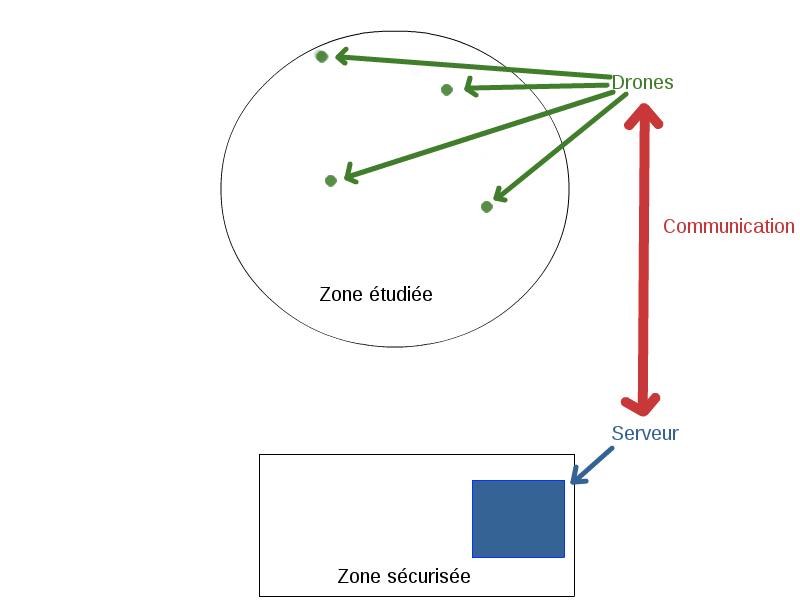
\includegraphics[scale=0.23]{img/projet_schema.png}
	\caption{Schéma du réseau}
      \end{figure}  
    \end{frame}
    
    \rmheader
    %Présenter vulgairement notre application
    \begin{frame}
      \frametitle{Introduction}
      \framesubtitle{Application}
      
      \begin{itemize}
	\item Drones autonomes et équipés d'un capteur ultrason
	\item Communication par fréquences radio
	\item Représentation graphique de la zone en temps réel
      \end{itemize}
    \end{frame}
  }
  
  %Plan de la présentation
  %Expliquer le déroulement de la présentation
  {
    \rmheader
    \begin{frame}
      \frametitle{Déroulement de la présentation}
      \tableofcontents[hidesubsections]
    \end{frame}
  }
  
  %Section Serveur
  %Présenter le serveur : de quoi il est constituer ? comment il fonctionne ? qu'est-ce qu'on obtient, etc...
  {
    \section{Serveur}
      
      %Sous-section Principe de fonctionnement
      %Présenter le schéma et le rôle de chaque tâche
      \subsection{Principe}
	\begin{frame}
	  
	\end{frame}

      %Sous-section Développement du serveur
      %Présenter l'implémentation de chaque tâche
      \subsection{Développement}
	\begin{frame}
	
	\end{frame}
	
      %Sous-section Démonstration du fonctionnement
      %Montrer une impression d'écran de topographie et faire une démonstration en direct
      \subsection{Démonstration}
	\begin{frame}
	 
	\end{frame}
  }
  
  %Section Drone
  %Présenter le drone : Les composants, les librairies, le résultat final, ...
  {
    \section{Drone}
    
      %Sous-section
      \subsection{Étude préliminaire}
	\begin{frame}
	  
	\end{frame}
      
      \subsection{Nos composants}
	\begin{frame}
	 
	\end{frame}

      
      \subsection{Le montage}
	\begin{frame}
	 
	\end{frame}

      
      \subsection{Résultat final}
	\begin{frame}
	 
	\end{frame}


  }
  
  %Section Analyse
  {
    \section{Analyse}
  }
  
  %Section Conclusion
  {
    \section{Conclusion}
  }
\end{document}
